\section{Evaluation}
\label{sec:eval}

We evaluated \tool and the LLMT algorithm behind it
 with two quantitative research questions and a third qualitative one:

\begin{enumerate}[label=RQ \arabic*.,ref=RQ \arabic*]
  \item Can \tool compress programs better than a state-of-the-art library learning tool?\label{rq:1}
  \item Are the main techniques in LLMT (anti-unification and equational theories)
        important to the algorithm's performance?\label{rq:2}
  \item Do the functions \tool learns make intuitive sense?\label{rq:3}
\end{enumerate}

\mypara{Benchmark Selection}
We use two suites of benchmarks to evaluate \tool, both shown in \autoref{tab:benchmarks}.
%
The first suite originates from the \dc work~\cite{dreamcoder},
 and is available as a public repository~\cite{compression-bench}.
\dc is the current state-of-the-art library learning tool,
and using these benchmarks allows us to perform a head-to-head comparison.
%
The \dc benchmarks are split into five domains (each with a different DSL);
we selected two of the domains---List and Physics---which we understood best,
to add an equational theory.

The second benchmark suite, called \cogsci, comes from \citet{cogsci-dataset}.
This work collects a large suite of programs in a graphics DSL for the
 purpose of studying connections between the generated objects and their
 natural language descriptions.
There are 1,000 programs in the ``Drawings'' portion of this dataset,
 divided into four subdomains (listed in \autoref{tab:benchmarks})
 of 250 programs each.\looseness=-1
%For use in \tool,
% we combine each suite of 250 programs into a large single benchmark
% from which to learn libraries.

We ran \tool on all benchmarks on an AMD EPYC 7702P processor at 2.0 GHz.
Each benchmark was run on a single core.
The \dc results were taken from
 the benchmark repository~\cite{compression-bench};
 \dc was run on 8 cores of an AMD EPYC 7302 processor at 3.0 GHz.

%Times for \dc were taken from \citet{dreamcoder}
%  as we were unable to run \dc,
%  much less reproduce their results,
%  even after multiple consultations with the authors.
%\mw{should we say we can't run \dc? is this too aggressive?}

% %
% Describe the two benchmark suites: \dc and \cogsci.
% %
% Explain the subtlety that for the \dc benchmarks we want to compress the minimal solution
% to each synthesis problem, and how we handle that
% (we put different solutions into the same e-class).
% %
% Explain the role of the \cogsci domain: these are benchmarks with more and larger programs,
% which \dc cannot handle.

\begin{table}
  \centering
  \begin{tabular}{lrr}
    \multicolumn{3}{c}{\dc~\cite{dreamcoder}} \\
    \bf Domain & \bf \# Benchmarks & \bf \# Eqs \\
    List    & 59 & 14 \\
    Physics & 18 & 8 \\
    Text    & 66 & - \\
    Logo    & 12 & - \\
    Towers  & 18 & -
  \end{tabular}\qquad%
  \begin{tabular}{lrr}
    \multicolumn{3}{c}{\cogsci~\cite{cogsci-dataset}} \\
    \bf Domain & \bf \# Benchmarks & \bf \# Eqs \\
    Nuts \& Bolts & 1 & 7 \\
    Vehicles      & 1 & 9 \\
    Gadgets       & 1 & 17 \\
    Furniture     & 1 & 9 \\
    & %dummy line
  \end{tabular}
  \caption{
    We selected our benchmark domains from two previous works:
     \dc~\cite{dreamcoder}
     and \cogsci~\cite{cogsci-dataset}.
    Each domain from \dc has multiple benchmarks;
     \cogsci has one large benchmark per domain.
    For some domains,
     we additionally supplied \tool with an equational theory;
     we report the number of equations in the final column.
  }\label{tab:benchmarks}
\end{table}

\subsection{Comparison with \dc}

\begin{figure}
  \centering
  \begin{subfigure}{0.48\linewidth}
    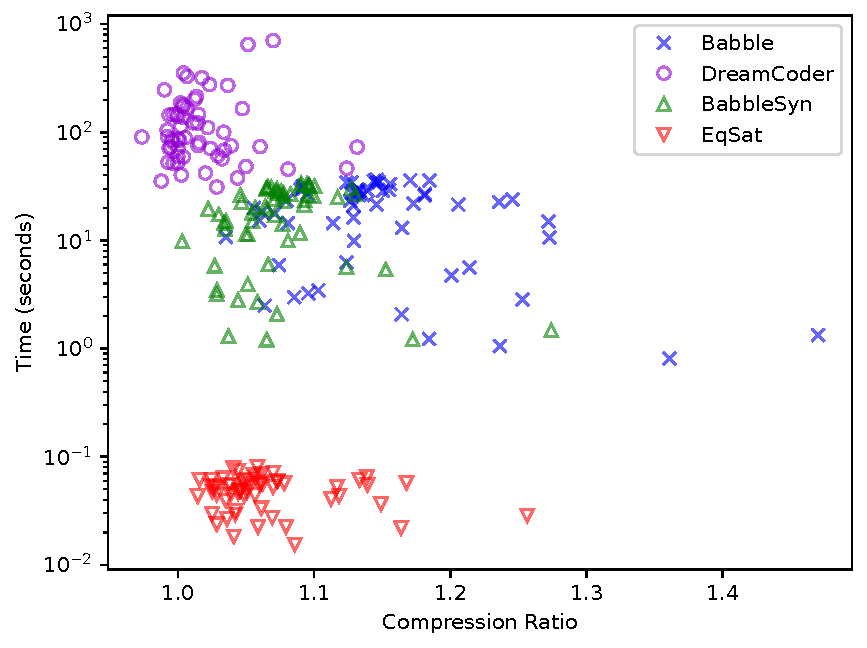
\includegraphics[width=\linewidth]{figures/scatter/list.pdf}
    \caption{List domain}
    \label{fig:dc-domains-list}
  \end{subfigure}
  \hfill
  \begin{subfigure}{0.48\linewidth}
    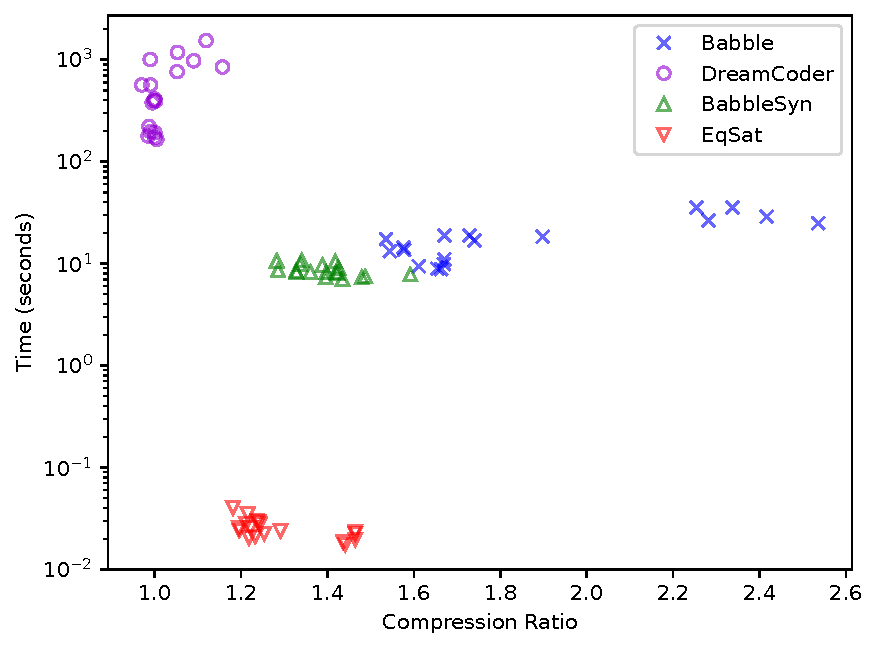
\includegraphics[width=\linewidth]{figures/scatter/physics.pdf}
    \caption{Physics domain}
    \label{fig:dc-domains-physics}
  \end{subfigure}

  \begin{subfigure}{0.48\linewidth}
    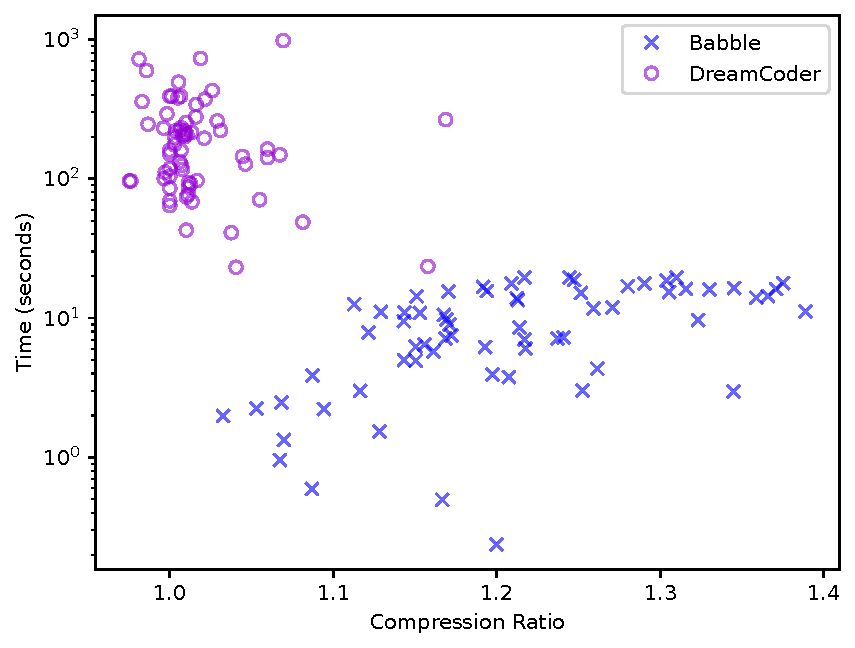
\includegraphics[width=\linewidth]{figures/scatter/text.pdf}
    \caption{Text domain}
  \end{subfigure}
  \hfill
  \begin{subfigure}{0.48\linewidth}
    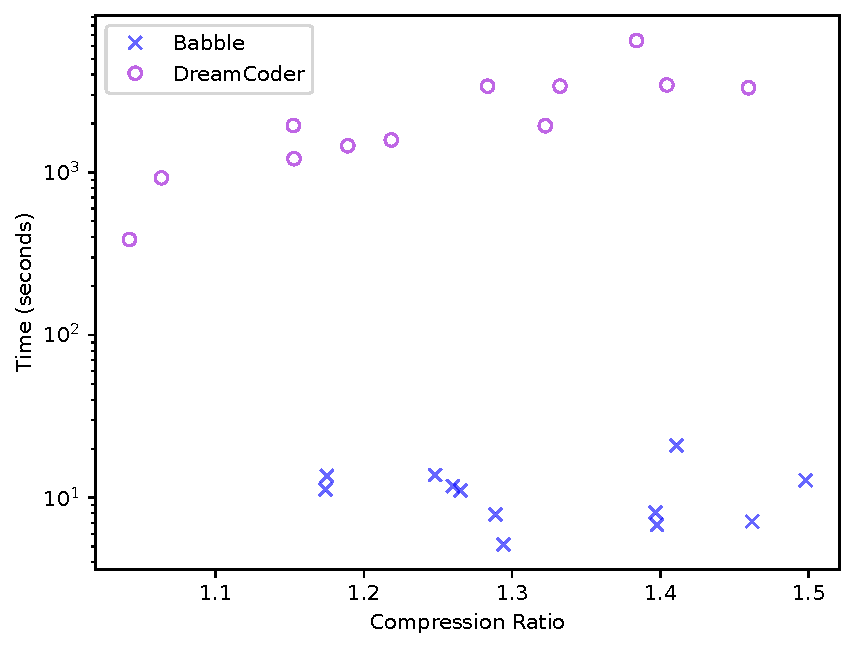
\includegraphics[width=\linewidth]{figures/scatter/logo.pdf}
    \caption{Logo domain}
  \end{subfigure}

  \begin{subfigure}{0.48\linewidth}
    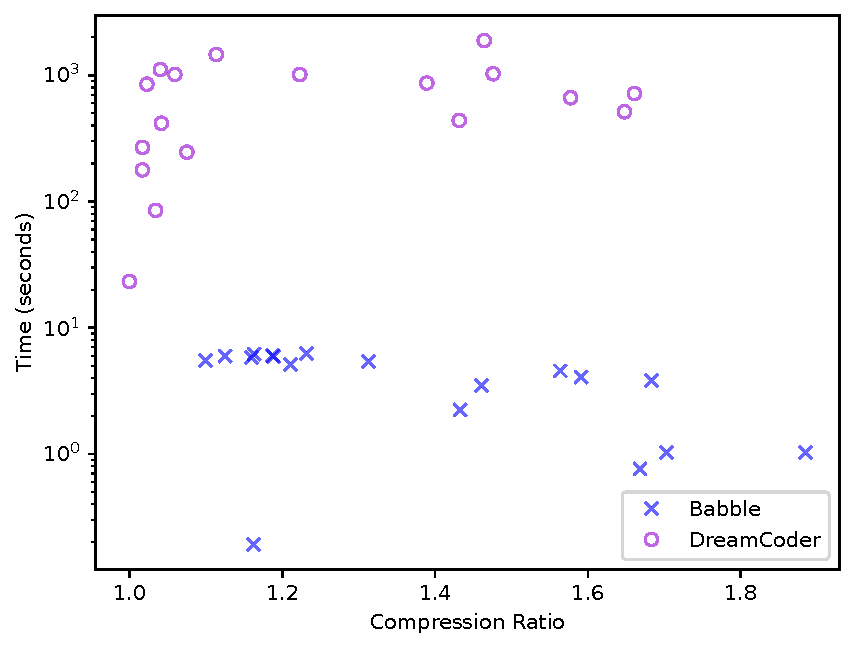
\includegraphics[width=\linewidth]{figures/scatter/towers.pdf}
    \caption{Towers domain}
  \end{subfigure}
  \caption{
    \tool consistently achieves better compression ratios than
     \dc on benchmarks from the \dc domains,
     and it does so 1--2 orders of magnitude faster.
    Each marker shows the compression ratio (x-axis)
     and run time (y-axis) of a benchmark.
    Each benchmark is one \dc input,
     \ie, a set of groups of programs as described above.
    Lower and to the right is better.
    In the domains where we supplied
     \tool with an equational theory
     (List and Physics),
     additional markers show the performance
     of \tool using purely syntactic learning (without equations, ``BabbleSyn'')
     or only equality saturation without library learning (``EqSat'').
  }\label{fig:dc-domains}
\end{figure}

To answer \ref{rq:1},
 we compare to the state-of-the-art \dc tool~\cite{dreamcoder} on its own benchmarks.
The \dc benchmarks are suited to its workflow;
while the input to a library learning task
 is conceptually a set of programs (or just one big program),
 each input to \dc is a set of \emph{groups} of programs.
Each group is a set of programs
 that are all output from the same program synthesis task
 (from an earlier part of the \dc pipeline).
When compressing a program via library learning,
 \dc is minimizing the cost of the program
 made by concatenating the most compressed
 program from each group together, in other words:
\[
  \sum_{\textsf{group $g$}}
  \min_{\textsf{program $p \in g$}}
  \textsf{cost}(p)
\]
\dc takes this approach to give its library learning
 component many variants of the same program,
 in order to introduce more shared structure
 between solution programs across different synthesis problems.
 %in hopes that some variants will compress better than others in different contexts.
 %\mw{someone who understands dc should check me on this}

To implement \dc's benchmarks in \tool,
 we use the \egraph to capture the notion of program variants in a group.
Since every program in a group is the output of the same synthesis task,
 \tool considers them equivalent and places them in the same \eclass.

% The input to each library learning task
%  is a set $P$ of sets of programs:
% \[
%   P = \{
%     \{p_{1,1}, p_{1,2}, \ldots \},
%     \{p_{2,1}, p_{2,2}, \ldots \},
%     \{p_{3,1}, p_{3,2}, \ldots \},
%     \ldots
%   \}
% \]
% Let $p_i = \{p_{i,j} \mid j\}$ refer to an inner set of programs.
% Each program in a set $p_i$
%  is the output from the same synthesis task.


\mypara{Results}
We ran \tool on five domains from the \dc benchmark suite.
The results are shown in \autoref{fig:dc-domains}.
In summary,
 \tool consistently achieves better compression ratios than
 \dc on benchmarks from the \dc domains,
 and it does so 1--2 orders of magnitude faster.


% without any DSRs.
% %
% Show that we get better compression
% \TODO{even if we run for as many rounds as \dc?}
% %
% Say something about time/memory to show that we are not much slower than DC.

\mypara{The Role of Equational Theory}
\label{sec:ablation}
%
To answer \ref{rq:2},
 we again turn to the \dc benchmarks,
 focusing on the domains where we supplied \tool
 with an equational theory: List and Physics.
In these domains, we ran \tool in two additional configurations:
\begin{itemize}
  \item ``BabbleSyn'' ignores the equational theory, just doing syntactic library learning.
  \item ``EqSat'' just optimizes the program using Equality Saturation with the
        rewrites from the equational theory.
        This configuration \emph{does not} do any library learning.
\end{itemize}
\autoref{fig:dc-domains-list} and \ref{fig:dc-domains-physics}
 show the results for these additional configurations,
 as well as \dc and the normal \tool configuration.
All \tool configurations rely on
  targeted subexpression elimination
  to select the final learned library.
The ``EqSat'' configuration is unsurprisingly very fast
 but performs relatively little compression,
 as it does not learn any library abstractions.
The ``BabbleSyn'' configuration
 does indeed compress the inputs,
 in fact it is still better than \dc in both domains.
However,
 the addition of the equational theory (the ``\tool'' markers in the plots)
 significantly improves compression
 and adds relatively little run time,
 well within an order of magnitude.

\subsection{Large-Scale \cogsci Benchmarks}

\begin{table}
  \begin{tabular}{lr|rrr|rrr}
    \multicolumn{2}{c}{} & \multicolumn{3}{c}{Without Eqs} & \multicolumn{3}{c}{With Eqs} \\
    \bf Benchmark & \bf Input Size & \bf Out Size & \bf CR & \bf Time (s) & \bf Out Size & \bf CR & \bf Time (s) \\
    Nuts \& Bolts   &      19009 &       2059 &       9.23 &      18.74 &       1744 &      10.90 &      40.75 \\
    Vehicles        &      35427 &       6477 &       5.47 &      79.50 &       5505 &       6.44 &      78.03 \\
    Gadgets         &      35713 &       6798 &       5.25 &      75.07 &       5037 &       7.09 &      82.29 \\
    Furniture       &      42936 &      10539 &       4.07 &     133.25 &       9417 &       4.56 &     110.00 \\
    \hline
    Nuts \& Bolts (clean) & 18259 &       2215 &       8.24 &      18.12 &       1744 &      10.47 &      40.91
  \end{tabular}
  \vspace{1em}
  \captionof{table}{
    Results for running \tool on the four large examples
     from the \cogsci dataset~\cite{cogsci-dataset},
     both without and with an equational theory.
    Each row includes the input and output AST sizes,
     the compression ratio (CR),
     and \tool's run time in seconds.
    \autoref{fig:cogsci-scatter} plots this data.
    The final row shows performance on a modified dataset.
  }\label{tab:cogsci}
\end{table}
\begin{figure}
  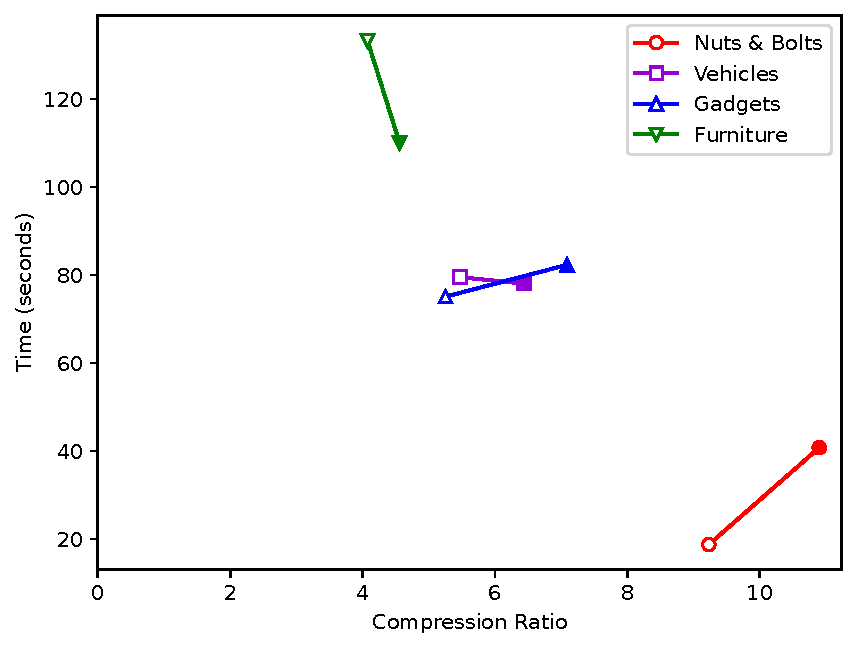
\includegraphics[height=5cm]{figures/scatter/cogsci-scatter.pdf}
  \caption{
    Data from \autoref{tab:cogsci} in scatter plot.
    Each line segment shows compression ratio and run time for a domain
     without (hollow marker) and with (solid marker) an equational theory.
    Using an equational theory improves compression in all cases,
     and even improves run time in two cases.
  }\label{fig:cogsci-scatter}
\end{figure}

The previous section demonstrated that \tool's performance
 far surpasses the state of the art.
In this section,
 we present and discuss the results
 of running \tool on benchmarks from the \cogsci domain.
These benchmarks,
 taken from \citet{cogsci-dataset},
 are significantly larger (roughly 10x - 100x)
 than those from the \dc dataset
 and out of reach for \dc.

\mypara{Quantitative Results}
\autoref{tab:cogsci} and \autoref{fig:cogsci-scatter} show the results
 of running \tool on the benchmarks from the \cogsci domain.
The plot in \autoref{fig:cogsci-scatter} makes two observations clear.
First and relevant for \ref{rq:2},
  the addition of an equational theory improved all four benchmarks
  (the solid marker is always to the right of the hollow marker).
Second, and perhaps surprisingly,
 equational theories can sometimes make \tool \emph{faster}!
This is consistent with previous observations about equality saturation~\cite{willsey2021egg}:
 while equality saturation typically makes an e-graph larger,
 it can sometimes combine two relevant e-classes into one and
 reduce the amount of work that some operation over an e-graph must do.

We also observed that the \nuts dataset contains
  several redundant transformations,
  like the ``scale by 1'' featured in the running example of \autoref{sec:overview}. %in \autoref{eq:unit-xform} and \autoref{fig:polygons}.
These redundancies can be useful for finding
  abstractions in the absence of an equational theory.
However, they should not be required in
  \tool since LLMT can
  introduce the redundancies wherever
  required.
We therefore removed all
  existing redundant transformations
  from \nuts and ran \tool
  on the transformed dataset.
The results are in the final row of \autoref{tab:cogsci}.
On the modified dataset,
 \tool achieves identical compression when using the equational theory,
 but without the equations it performs worse than on the unmodified dataset.

\mypara{Qualitative Evaluation}
\label{sec:quali}
%
\begin{figure}
  \centering
  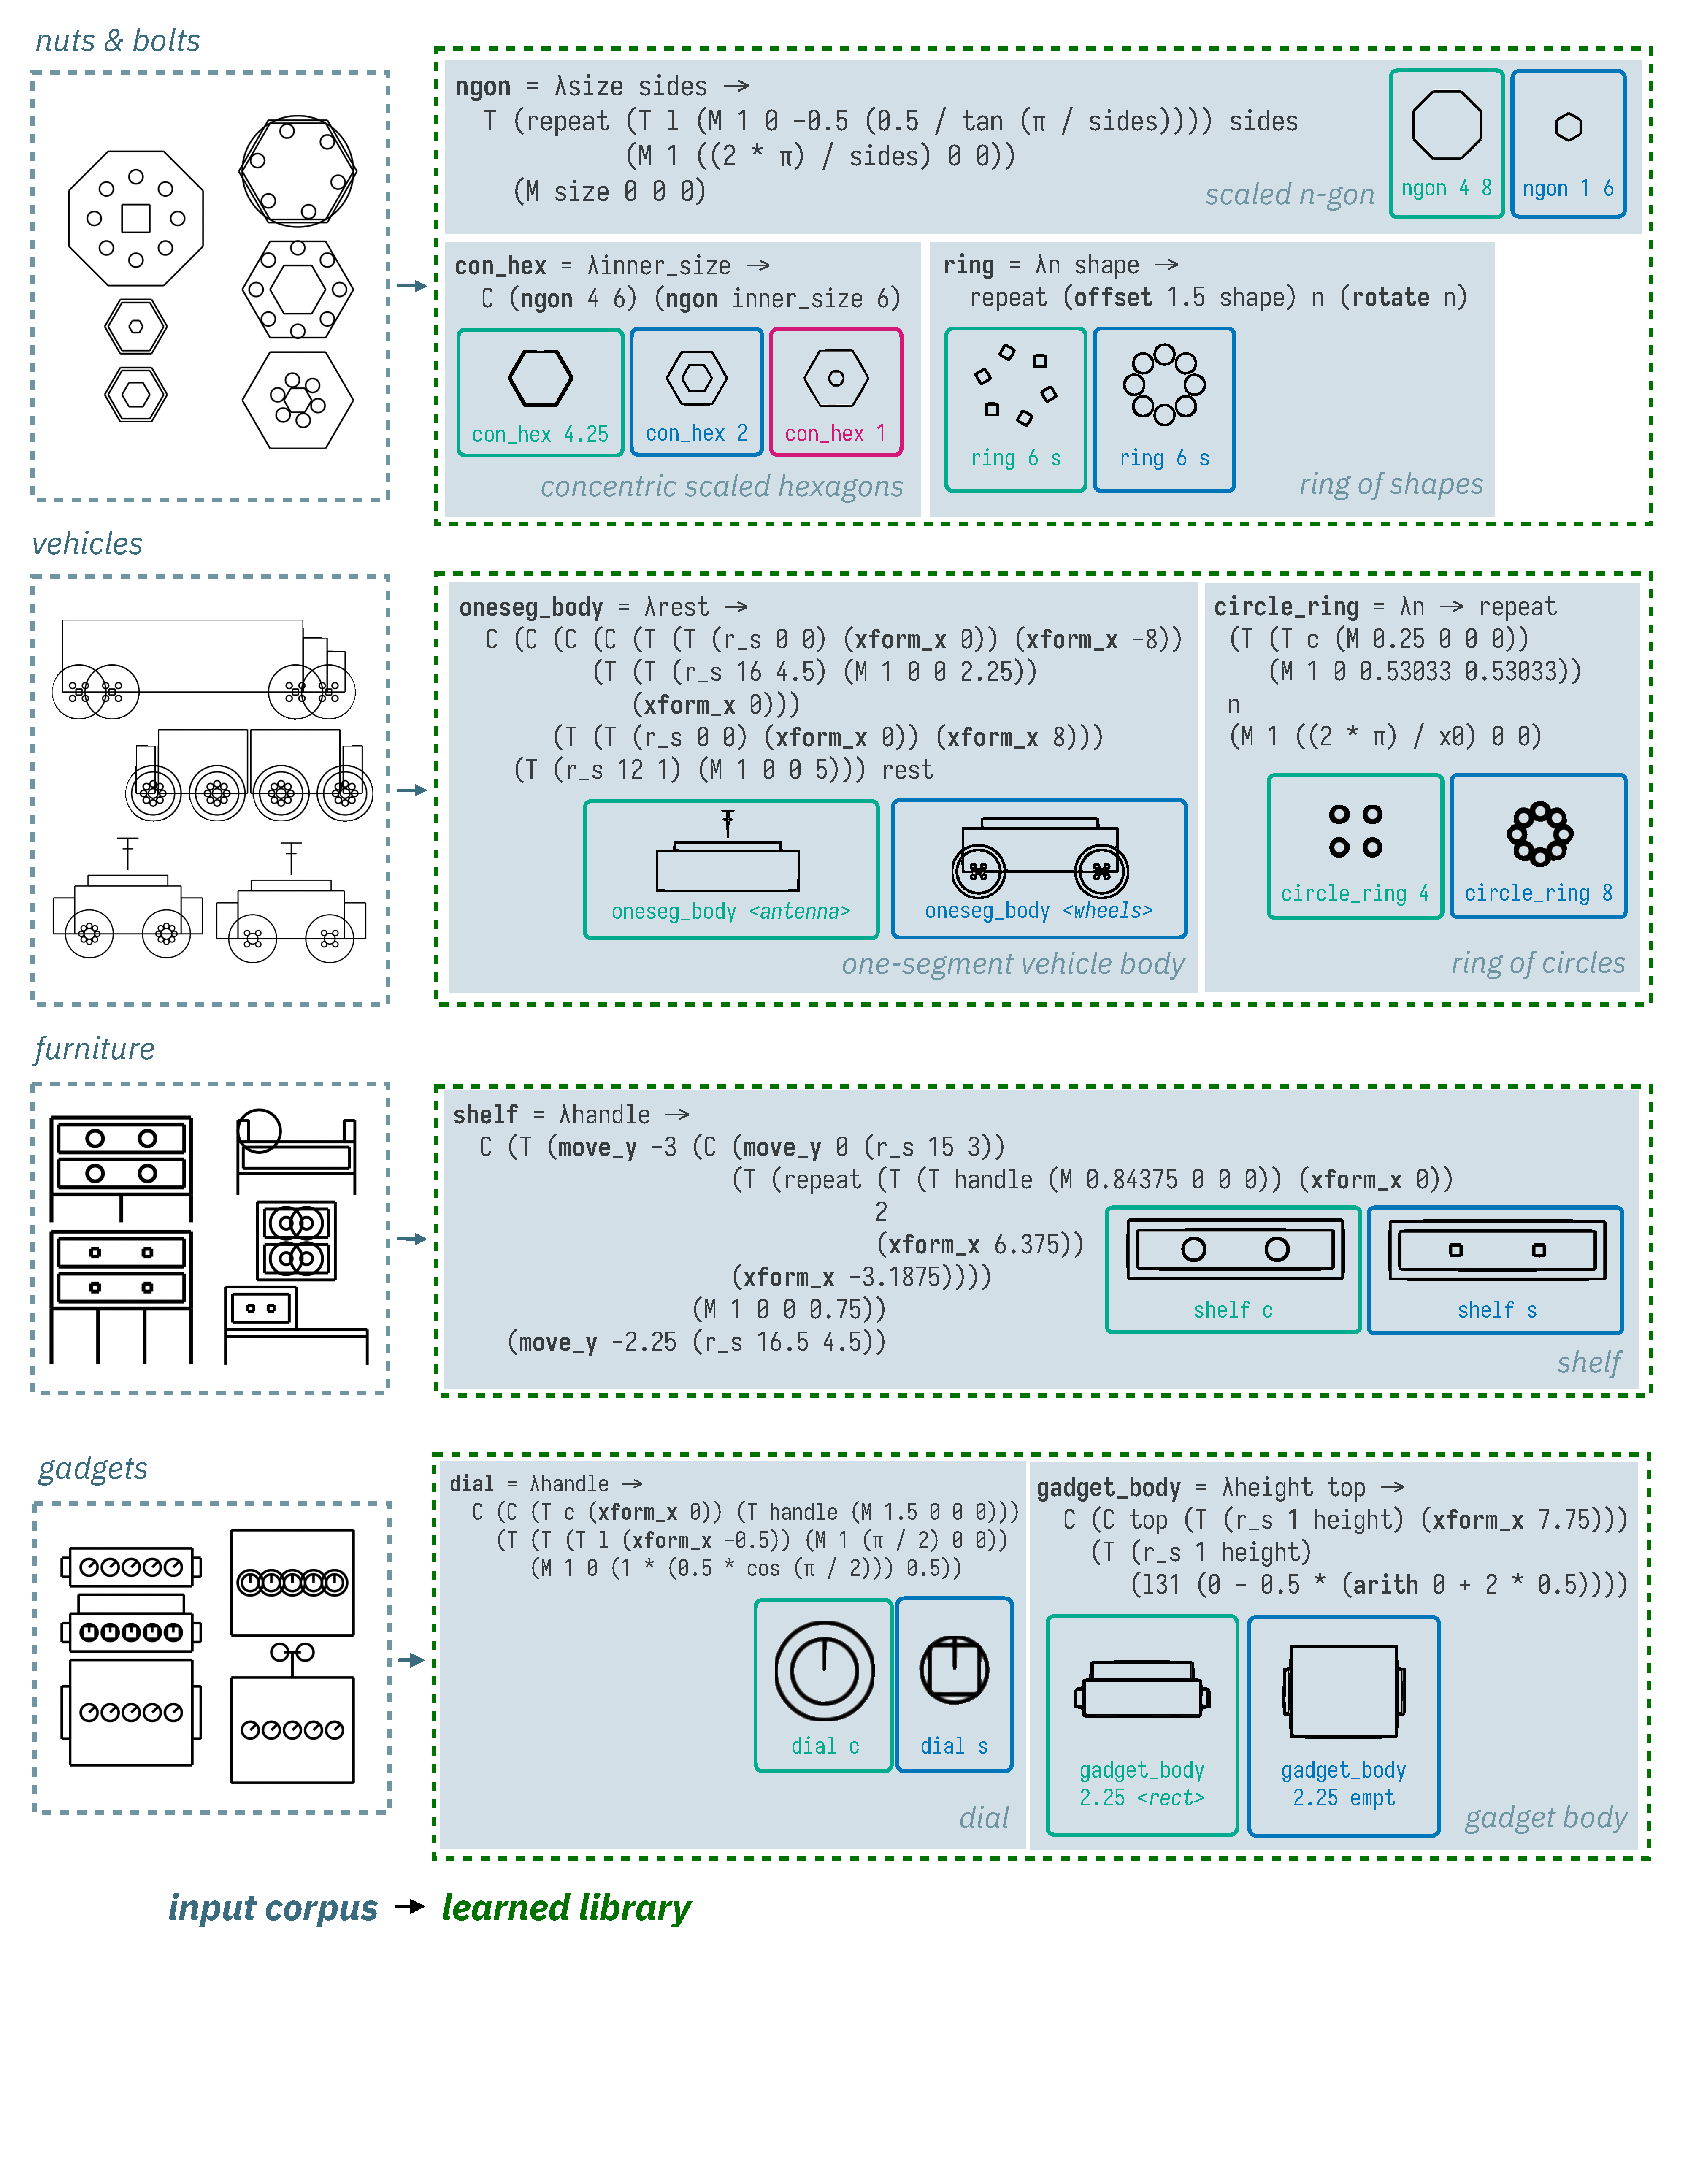
\includegraphics[width=\textwidth]{figures/qual_cogsci.pdf}
  \caption{A selection of evaluated programs from each of the domains
           in the \cogsci dataset, along with a selection of functions
           that \tool learns within the first ten rounds for each domain.
           Bolded functions represent learned abstractions.
           Note this figure uses the concrete syntax from the \cogsci
           dataset; it is similar to the simplified form shown in the overview.
           We named the learned functions and their parameters for clarity.
   }\label{fig:qual_cogsci}
\end{figure}
%
\autoref{fig:qual_cogsci}
 highlights a sample of abstractions that
 \tool discovered from the \cogsci benchmarks.
We ran \tool on each of the benchmarks
  and applied the learned abstractions on a few input programs to
  visualize their usage.
Questions about usability and readability of
  learned libraries are difficult to answer
  without rigorous user studies which we leave for
  future work.
Nevertheless, \autoref{fig:qual_cogsci} shows that
  \tool identifies common structures that
  are similar across
  different benchmarks, which
  makes its output easier to reuse and interpret.

First, we revisit the \nuts example
  from \autoref{sec:intro}:
  \autoref{fig:qual_cogsci} shows that \tool %successfully
  learns the scaled polygon (\texttt{ngon}) abstraction which
  is applicable to several programs in the dataset.
We also see that \tool consistently
  finds a similar abstraction
  representing a ``ring of shapes'' for both
  \nuts and Vehicles.
Finally, as the Gadgets example shows,
  \tool finds abstractions for both
  the entire model as well as its components.
In this case,
  it learned the function \texttt{gadget\_body}
  that abstracts the entire outer shape,
  and it also learned \texttt{dial} that abstracts
  the handles of the outer shape.\looseness=-1
